\documentclass[12pt, 
hyperref={colorlinks=true, linkcolor=blue, urlcolor=cyan}]{beamer}
\usetheme{default} 

\setbeamertemplate{navigation symbols}{} %gets rid of navigation symbols
\setbeamertemplate{footline}{} %gets rid of bottom navigation bars
\setbeamertemplate{footline}[page number]{} %use this for page numbers

\setbeamertemplate{itemize items}[circle] %round bullet points
\setlength\parskip{10pt} % white space between paragraphs

\usepackage{wrapfig}
\usepackage{subfig}
\usepackage{setspace}
\usepackage{enumerate}
\usepackage{graphicx}
\usepackage{amsmath}
\usepackage{amsfonts}
\usepackage{amssymb}
\usepackage{amsthm}
\usepackage[UKenglish]{isodate}
\usepackage{color}
\cleanlookdateon

% the preamble
\title{BIOST 311: \\ Regression Methods for the Health Sciences}
\author{Kelsey Grinde and Brian Williamson}
\institute{UW Biostatistics}
\date{Spring 2018}
\begin{document}
% title slide
\begin{frame}
\titlepage\thispagestyle{empty}
\end{frame}

% do de-brief discusion section, mention index card grade, check that everyone has been able to knit, reminder about OH and HW
\begin{frame}
\frametitle{Checking in...}
\begin{itemize}
\item Yesterday's discussion section % everyone has submitted; don't worry about submission time -- just by end of day; grading is just credit/no credit; congrats on surviving day 1: everyone did REALLY well -- we're very impressed by how quickly you picked things up; we'll continue to work on this throughout the quarter, so it might feel like a lot right now but it will get easier!
	\begin{itemize}
	\item Congrats on creating your first R Markdown document!
	\item FYI: grading is credit/no credit
	\end{itemize}
\item Grades for index card 1 are posted % everyone has 100%! moving forward: grading is always credit/no credit; about once per week
	\begin{itemize}
	\item Future index cards/activities that you hand in for credit/no credit $\approx$ once/week
	\end{itemize}
\item Starting your \href{https://canvas.uw.edu/courses/1203588/assignments/4098142}{first assignment} % can you access? can you knit? after today, should be able to do everything; please don't save knitting until the last minute!
	\begin{itemize}
	\item Download the \texttt{.Rmd} file
	\item Update the author, output type, type in your answers % (should be able to answer everything after class today)
	\item \texttt{Knit} (try this early!) % if time, could do together at end of class
	\item Turn in .pdf/Word doc that gets created \textit{and} \texttt{.Rmd} file
	\end{itemize}
\item Questions? Come to office hours today (2--4) % check if time works for most people
\end{itemize}
\end{frame}


% make it 0.something
\setbeamertemplate{footline}{%
  \raisebox{5pt}{\makebox[\paperwidth]{\makebox[120pt]{\scriptsize Last updated \today}\hfill\makebox[10pt]{\scriptsize 0.\insertframenumber~~}}}}
\newcounter{chap0}{\value{1}}
\setcounter{framenumber}{\value{chap0}}

% Chapter 0 learning objectives
\begin{frame} 
\frametitle{CHAPTER 0: BIOST 310 REVIEW}
By the end of Chapter 0 you should be able to: \vspace{-0.2cm}
\begin{itemize}
\item Identify and describe common study designs
\item Classify variables according to their type (e.g., binary)
\item Use numerical and graphical tools to summarize data
\item Explain features of and calculate probabilities using important probability distributions (Normal, t)
\item Define a sampling distribution
\item State the Central Limit Theorem and understand its importance for statistical inference
\item Construct and interpret confidence intervals
\item Formulate null and alternative hypotheses
\item Choose, implement, and interpret hypothesis tests
\end{itemize}
\end{frame}

% Chapter 0 motivation
\begin{frame}
\frametitle{Why spend time reviewing these concepts?} % different courses, different instructors (and refresh for those for whom it's been awhile)
1. So everyone starts on the same page \\
2. These concepts are \textit{very} important for data analysis: \vspace{-0.35cm} % key components of data analysis
	\begin{itemize} \small \itemsep -0.5pt
	\item Understanding the data you have and its limititations: how (\textit{study design}) and what  (\textit{classifying variables}) was collected
	\item Converting your scientific questions into statistical ones (\textit{formulating hypotheses})
	\item Choosing appropriate statistical methods (based on $\uparrow$) 
	\item Summarizing your data (\textit{numerical and graphical summaries})
	\item \begin{footnotesize} (Most minor of all: running your chosen statistical methods) \end{footnotesize}
	\item Correctly interpreting your statistical results (\textit{parameter estimates, confidence intervals, p-values})
	\end{itemize}
\end{frame}

% Study design motivation
\begin{frame}
\frametitle{Study Design}
\textit{How you collect data impacts what questions you can (cannot) answer, what statistical methods you can (cannot) use, and what conclusions you can (cannot) draw.}

\color{blue} Extreme Example: \color{black} Suppose I'm interested in understanding public opinion about biostatistics. I  randomly select one individual from our class and ask if he/she likes biostatistics. \vspace{-0.3cm}

\begin{itemize} % this example is a bit contrived, but demonstrates some of why we care so much about study design
\item What questions can I answer using these data? 
\item What statistical methods can I use to analyze these data? 
\item What conclusions can I draw using these data? 
\end{itemize} 

\end{frame}

% types of study designs
\begin{frame}
\frametitle{Study Design: Experimental vs Observational}

\color{blue} Experimental: \color{black} exposure/treatment is \textit{controlled} by researcher (e.g., randomly assign people to drug or placebo) \vspace{-0.3cm}
	\begin{itemize}
	\item Randomized controlled trial % aka randomized control trial, randomized clinical trial
	\end{itemize}

\color{blue} Observational: \color{black} exposure/treatment is \textit{not controlled} by the researcher (e.g., we look at a group of people and \textit{observe} who smokes and who doesn't smoke)  \vspace{-0.3cm}
	\begin{itemize}
	\item Cross-sectional study
	\item Cohort study
	\item Case-control study
	\end{itemize}
\end{frame}

\begin{frame}
\frametitle{Study Design: Experimental vs Observational}

In \textit{experimental} studies, we can talk about \color{blue} \textit{causation}\color{black}. In \textit{observational} studies we  talk instead about \color{blue} \textit{association} \color{black}(because we worry about \color{blue} \textit{confounding}\color{black}). % we'll come back to this when we talk about interpreting results

A \color{blue} \textit{confounder} \color{black} is a variable that is causally associated with our outcome and also associated with the exposure in our sample. \vspace{-0.2cm}
\begin{itemize}
\item[] \textit{Example:} suppose we're interested in the relationship between smoking and lung function in kids. We know that age is causally associated with lung function: as children grow and develop, their lung function improves. If age is also associated with smoking in our sample (e.g., if older kids are more likely to smoke), then age is a confounder.
\end{itemize} 

\begin{small} \textit{Much more on this topic to come. Stay tuned!} \end{small}

\end{frame}

\begin{frame} % RCT
\frametitle{Experimental studies: randomized controlled trial}
Description:\vspace{-0.3cm}
\begin{itemize}
\item Take a sample of the population, \textbf{randomly assign} to treatment (\textit{exposed}) or control/placebo (\textit{unexposed}), and follow for disease outcomes (death yes/no, time to death)
\end{itemize}

\pause
Pros:\vspace{-0.3cm}
\begin{itemize}
\item With a large enough sample, no confounding!
\item Gold standard for establishing causality
\end{itemize}

\pause
Cons:\vspace{-0.3cm}
\begin{itemize}
\item Often very expensive
\item Not always possible or ethical to randomize
	\begin{itemize}
	\item Can't randomize sex, race, age, genetic variants
	\item Unethical to randomize to harmful exposures % e.g., smoking (FEV data), pollution (air pollution)
	\end{itemize}
\end{itemize}
\end{frame}

\begin{frame}
\frametitle{Experimental studies: randomized controlled trial}
Examples:
\begin{itemize}
\item \href{https://jamanetwork.com/journals/jama/article-abstract/2613159}{Effect of Vitamin D and Calcium Supplementation on Cancer Incidence in Older Women}
\item \href{http://stroke.ahajournals.org/content/36/8/1764.short}{Daily Functioning and Quality of Life in a Randomized Controlled Trial of Therapeutic Exercise for Subacute Stroke Survivors}
\end{itemize}
\end{frame}

% cross-sectional studies
\begin{frame}
\frametitle{Observational studies: cross-sectional study}
Description: \vspace{-0.3cm}
\begin{itemize}
\item Randomly sample individuals, record their exposure and outcome at a \textit{single time point} (no follow-up) % take a snapshot, taking a cross-section of the population
\end{itemize}

\pause
Pros:\vspace{-0.3cm}
\begin{itemize}
\item Relatively cheap and easy
\item Can study multiple outcomes and exposures % easy to collect a lot of data on each pers
\end{itemize}

\pause
Cons:\vspace{-0.3cm}
\begin{itemize}
\item Inefficient for rare exposure or disease % you won't have very many (or any) people in your sample with the thing you're interested in
\item Time sequence of exposure and outcome (i.e., which came first) is not always clear % did low exercise lead to obesity, or obesity lead to low exercise?
\item Potential confounding (so no conclusions about causality)
\end{itemize}
\end{frame}

\begin{frame}
\frametitle{Observational studies: cross-sectional study}
Examples:
\begin{itemize}
\item \href{http://ajph.aphapublications.org/doi/abs/10.2105/AJPH.78.10.1336}{Job strain, work place social support, and cardiovascular disease in a random sample of the Swedish working population}
\item \href{onlinelibrary.wiley.com/doi/10.1111/add.12623/full}{Real-world effectiveness of e-cigarettes when used to aid smoking cessation}
\end{itemize}
\end{frame}


% cohort studies
\begin{frame}
\frametitle{Observational studies: cohort study}
Description: \vspace{-0.3cm}
\begin{itemize}
\item Sample \textit{people without the outcome} (sometimes based on exposure, sometimes random), record their exposure, then \textit{follow} those individuals and see who gets outcome % often called longitudinal cohort study, often outcome is death
\end{itemize}

\pause
Pros:\vspace{-0.3cm}
\begin{itemize}
\item Time sequence is known (exposure came first)
\item Can study multiple outcomes 
\end{itemize}

\pause
Cons:\vspace{-0.3cm}
\begin{itemize}
\item Inefficient for rare outcomes % have to wait a lont time to get enough people with disease
\item Often expensive and time-consuming to follow people, and oppportunities for people to drop out
\item Potential confounding (so no conclusions about causality)
\end{itemize}
\end{frame}

\begin{frame}
\frametitle{Observational studies: cohort study}
Examples:
\begin{itemize}
\item \href{https://www.medicalnewstoday.com/articles/316619.php}{Drinking tea could help stave off cognitive decline}
\item \href{https://www.medicalnewstoday.com/articles/316565.php}{Birth control pills may protect against some cancers for decades}
\end{itemize}
\end{frame}

% case-control studies
\begin{frame}
\frametitle{Observational studies: case-control study}
Description: \vspace{-0.3cm}
\begin{itemize}
\item \textit{Sample individuals based on the outcome} (some with, some without), look back in time (usually) for exposure % when you look back in time = retrospective case-control study
\end{itemize}

\pause
Pros:\vspace{-0.3cm}
\begin{itemize}
\item Efficient for rare diseases % (don't have to recruit as many people)
\item Cheaper and faster than cohort studies
\item Can study multiple exposures
\end{itemize}

\pause
Cons:\vspace{-0.3cm}
\begin{itemize}
%\item Recall bias
\item May not know time sequence of disease and exposure
\item Cannot use to estimate relative risk or disease prevalence
\item Potential confounding (so no conclusions about causality)
\end{itemize}
\end{frame}

\begin{frame}
\frametitle{Observational studies: case-control study}
Examples:
\begin{itemize}
\item \href{https://www.sciencedirect.com/science/article/pii/S0140673605676635}{Obesity and the risk of myocardial infarction in 27,000 participants from 52 countries}
\item \href{http://www.nejm.org/doi/full/10.1056/NEJMoa065497\#t=article}{Case control study of human papillomavirus and oropharyngeal cancer}
\end{itemize}
\end{frame}

% let's practice
\begin{frame}
\frametitle{Study Design: Let's practice!}

Recent (June 2017) \href{http://www.nejm.org/doi/10.1056/NEJMoa1702747}{air pollution study} that has received a lot of attention in the news: \vspace{-0.3cm}
\begin{itemize} % headlines
\item ``U.S. air pollution still kills thousands every year, study concludes" -- NPR
\item ``Even 'safe' pollution levels can be deadly" --- NYT
\end{itemize}

From the article: \textit{We conducted a nationwide ... study involving all Medicare benficiaries from 2000 through 2012, a population of 61 million, with 460 million person-years of follow-up.}

\begin{small} \color{blue} What kind of study design is this? Why do you think they chose this design? What are potential limitations of this study design? \color{black} \end{small} % (think/write $\rightarrow$ pair $\rightarrow$ share). NOTE: this is the type of thing you'll need to be able to do on HW/exams
\end{frame}

% types of variables (brief reminders before we get to summarizing data)
\begin{frame}
\frametitle{Summarizing Data (Step 1): Types of Variables} % why do we care

\textit{How you summarize/analyze your data often depends on what type of data you've collected.} 

So, the first step to summarizing/describing your data is making sure you know what kind of data you have!

\color{blue} Extreme Example: \color{black} Suppose I'm intereseted in summarizing one of the variables in our FEV dataset: smoking habits (smoker/nonsmoker).  What numerical summaries can I use to get a sense of ``typical" smoking habits in our study? \vspace{-0.3cm}
\begin{itemize} % sketch what it looks like on board (note for future reference: this example needs more work)
\item Mean/average \pause \color{red} (No) \color{black}
\item Median \pause \color{red} (No) \color{black}
\item Mode \pause \color{red} (Yes) \color{black}
\item Proportion in each category \pause \color{red} (Yes) \color{black}
\end{itemize}
\end{frame}

\begin{frame}
\frametitle{Summarizing Data (Step 1): Types of Variables}

\color{blue} Categorical: \color{black} limited number of possible values
\begin{itemize}
\item \textit{Nominal:} order doesn't matter (e.g., blood type)
\item \textit{Ordinal:} order does matter (e.g., level of education)
\item \textit{Binary:} two possible values; nominal or ordinal (e.g., sex)
\end{itemize}

\color{blue} Quantitative: \color{black} infinite possible values
\begin{itemize}
\item \textit{Discrete:} values are integers; often counts (e.g., \#  teeth)
\item \textit{Continuous:} values on continuum (e.g., height)
\end{itemize}
\end{frame}


% Air pollution activity
\begin{frame}
\frametitle{Summarizing Data: Activity}

Let's read (parts of) the \href{http://www.nejm.org/doi/10.1056/NEJMoa1702747}{Di et al., ``Air pollution and mortality in the Medicare population."} paper. \vspace{-0.2cm}

\begin{enumerate}
\item Read: Abstract, Results (``Cohort Analyses" -- Figure 1)
\item Write down answers to the following questions:
	\begin{enumerate}
	\item What scientific question does this study address?
	\item List 3 variables that the authors collected and record their type.
	\item How did the authors summarize their data? (e.g., What numerical summaries did they present? How were they displayed? What graphical summaries did they present?)
	\item Is there any information that you wish they would have provided in their summary but did not?
	\end{enumerate}
\item Discuss with your neighbor, prepare to share
\end{enumerate}
\end{frame}

% sidebar: advertise Francesca's talk tomorrow
\begin{frame}
\frametitle{Think this research is interesting?}

One of the senior authors, \href{https://sites.sph.harvard.edu/francesca-dominici/}{Francesca Dominici}, is coming to campus this week as one of three finalists to be the next Dean of the School of Public Health!

Dr. Dominici will be giving a talk, titled ``How Data, Technology, and Infectious Optimism can Shape the Future of Public Health," at 3pm on Thursday (March 29) in HUB 332.

Details about each of the finalists and links to the livestreams of their talks \href{http://www.washington.edu/provost/leadership-searches/deanship-of-the-school-of-public-health/}{here}.
\end{frame}

% summarizing data, why do we care? (human genome example)
\begin{frame} 
\frametitle{Summarizing Data: Motivation}
\textit{Why is it so important to know how to summarize data?} \\ One answer: because we can't look at all of it, but we still want to make sense of it and draw conclusions from it.

\color{blue} Extreme example: \color{black} The Human Genome
\vspace{-0.4cm} \begin{center} 
\includegraphics[height=4cm]{./dna} \end{center}
\vspace{-0.8cm} \begin{scriptsize} A single human DNA sequence consists of $\approx$ 3 billion A's, C's, T's, and G's. \end{scriptsize}
\end{frame}

% human genome example (cont)
\begin{frame}
\frametitle{Summarizing Data: The Human Genome}
If we were to write out one human DNA sequence in \begin{tiny} tiny \end{tiny} font, what would that look like? 

\center 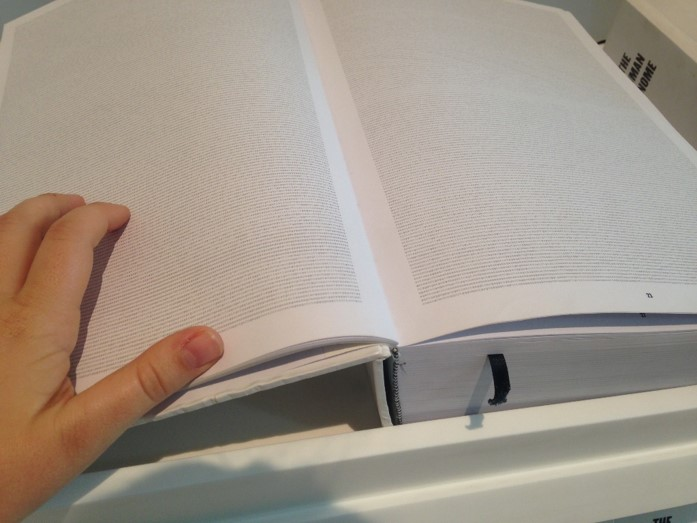
\includegraphics[height=4cm]{./book}

How many pages will it take? How many books?
\end{frame}

% human genome example (cont)
\begin{frame}
\frametitle{Summarizing Data: The Human Genome}
\vspace{-0.5cm}
\center 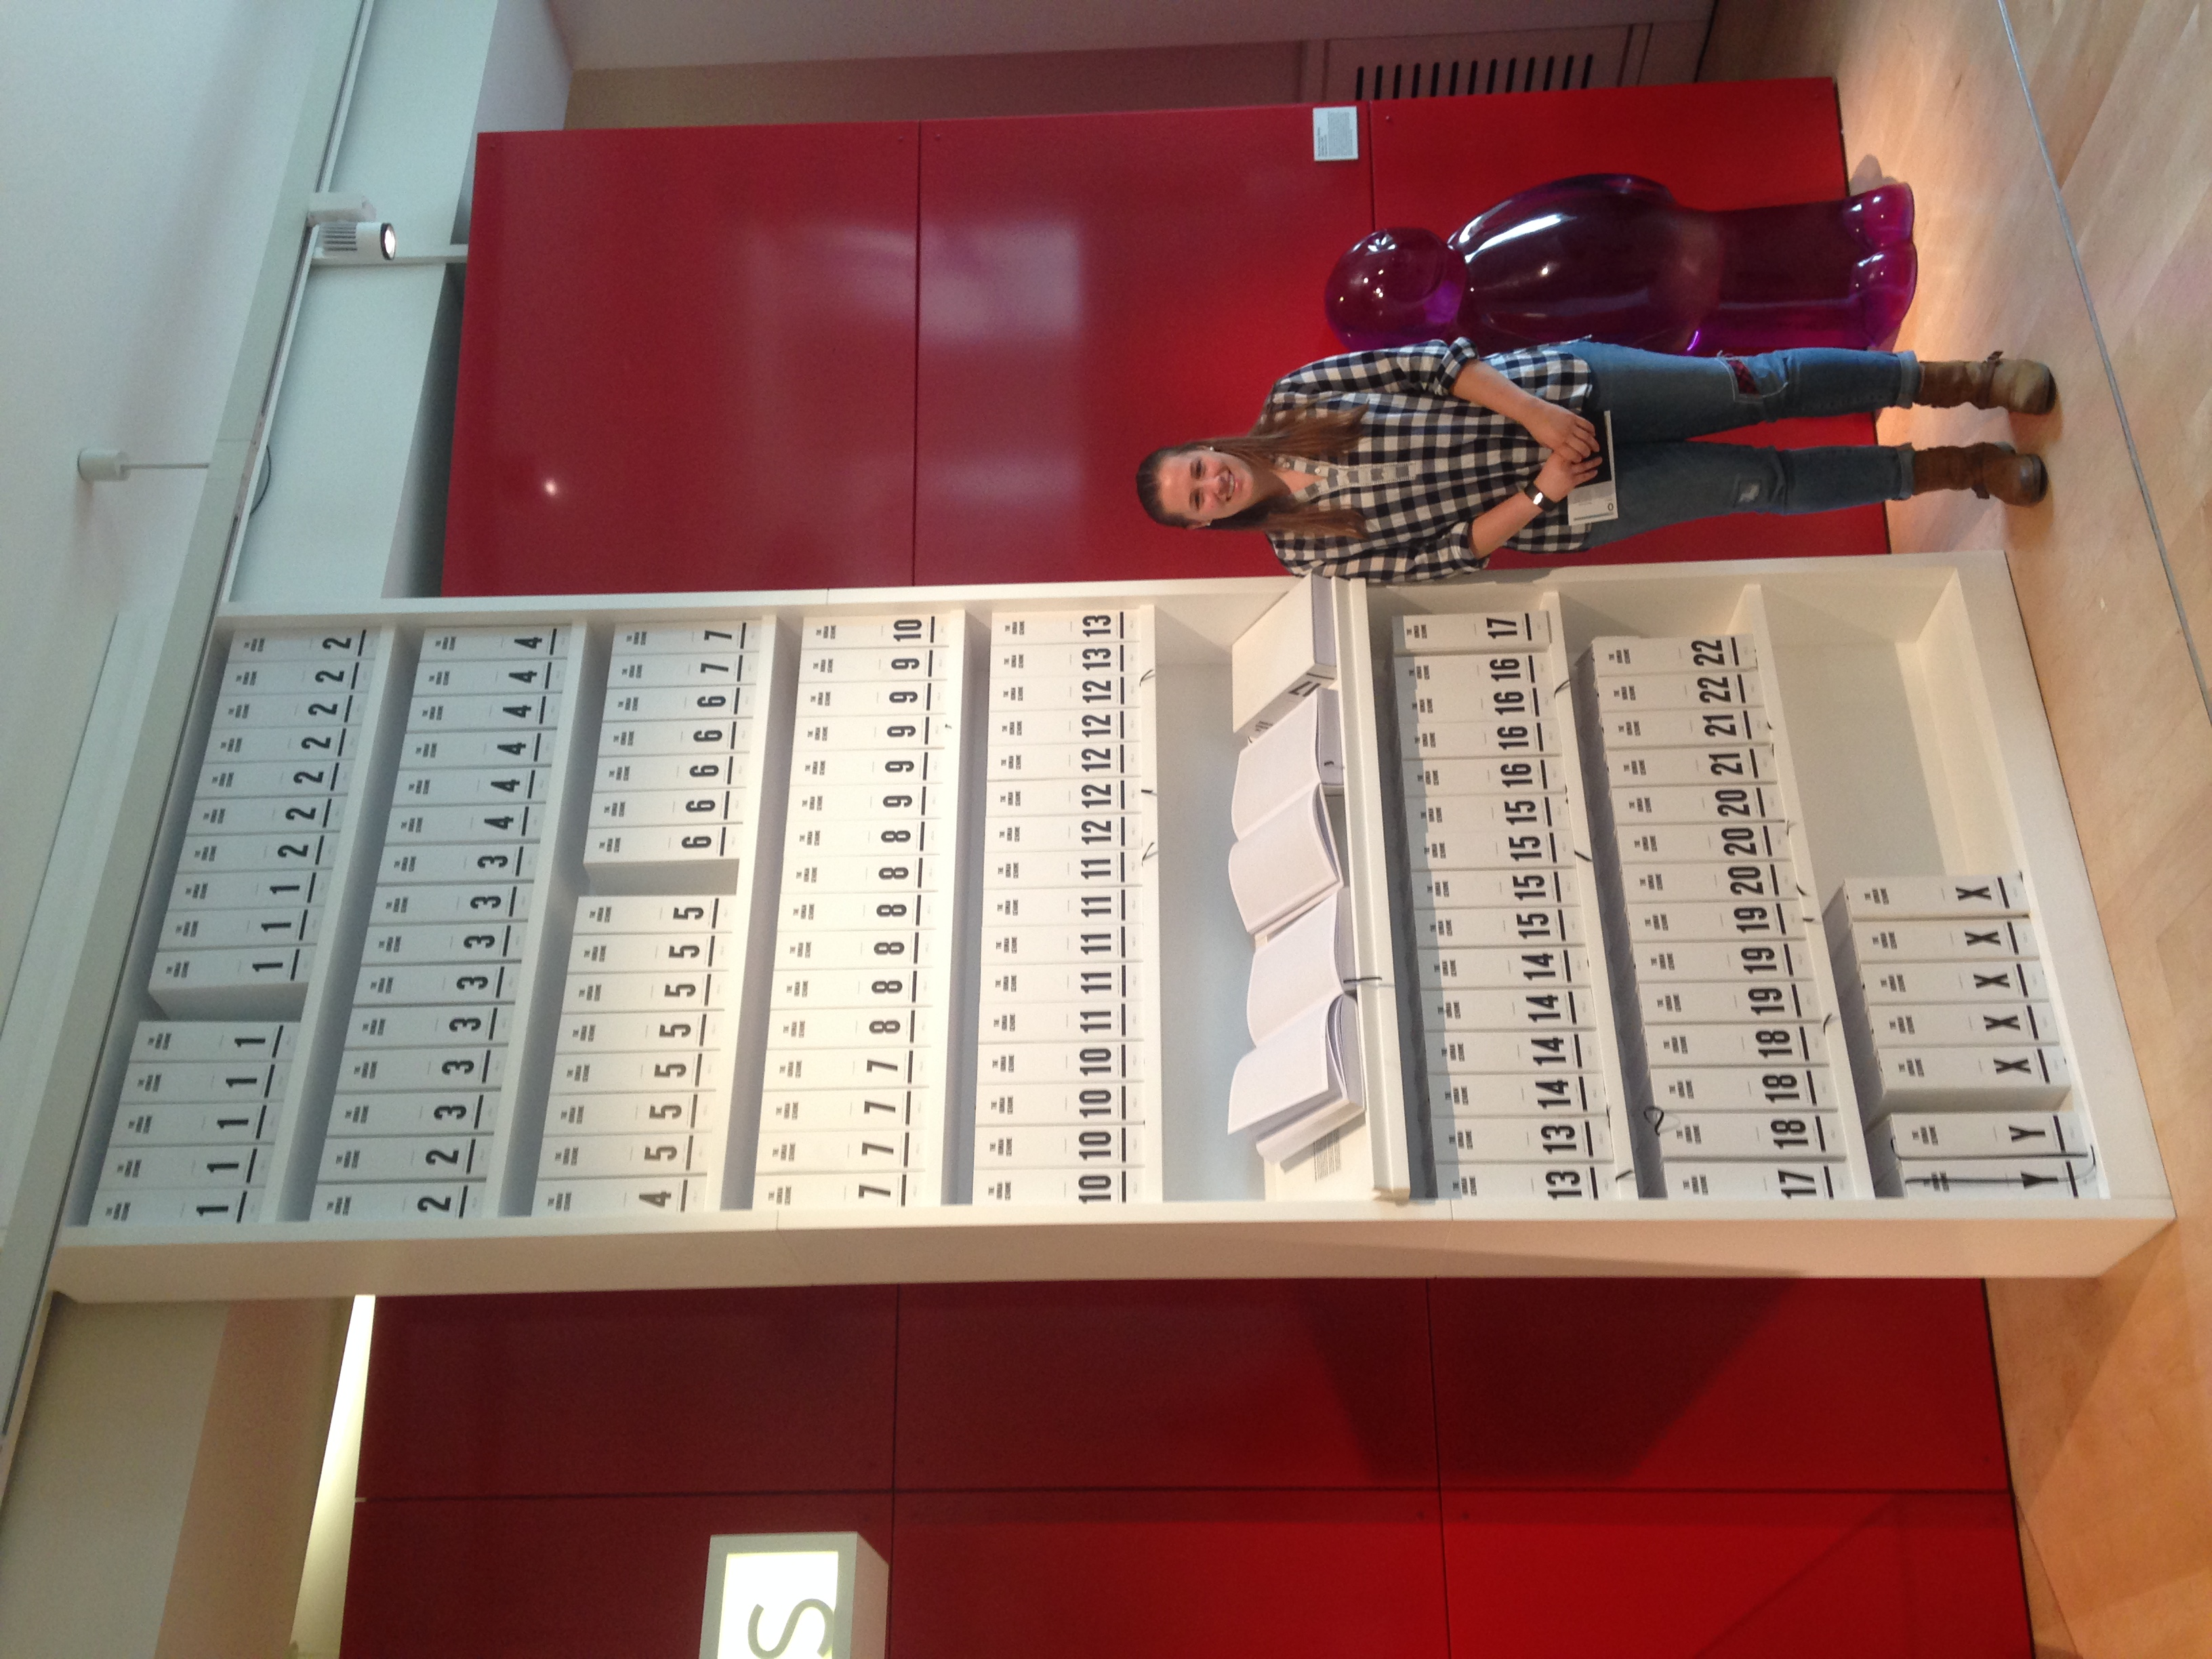
\includegraphics[height=0.65\textheight, angle = 270]{./bookcase}
\end{frame}

% why do we need descriptive stats
\begin{frame}
\frametitle{Summarizing Data: Descriptive Statistics}
Why do we need descriptive statistics?\vspace{-0.2cm}
\begin{itemize}
\item Making sense of large amounts of data
\item Checking data quality
	\begin{itemize}
	\item Values outside reasonable range \begin{footnotesize} (e.g., height = 9') \end{footnotesize}
	\item Implausible combinations of variables \begin{footnotesize} (e.g., pregnant men) \end{footnotesize}
	\end{itemize}
\item Observe distribution of variables in dataset
	\begin{itemize}
	\item Measures of center and spread
	%\item Skewness
	\end{itemize}
\item Start to understand direction and strength of association
	\begin{itemize}
	\item Descriptive statistics and inferential statistics should contribute to the same story
	\end{itemize}
\end{itemize}
\end{frame}

% types of descriptive statistics
\begin{frame}
\frametitle{Descriptive Statistics: Outline}

\begin{itemize}
\item Univariate
	\begin{itemize}
	\item Numerical (categorical variables)
	\item Numerical (quantitative variables)
	\item Graphical
	\end{itemize}
\item Stratified/Bivariate
	\begin{itemize}
	\item Numerical summaries, broken down by subgroup
	\item Graphical
	\end{itemize}
\end{itemize}

\end{frame}

% numerical descrip for categorical variables
\begin{frame}
\frametitle{Univariate Descriptive Statistics: Categorical}

Summary should include:
\begin{itemize}
\item Number and percent in each group
	\begin{itemize}
	\item If outcome of interest is binary, make sure to mention number of events
	\end{itemize}
\item If binary, only need to summarize one group
	\begin{itemize}
	\item The other can be inferred
	\end{itemize}
\item Also good to summarize missing data
	\begin{itemize}
	\item e.g., \#  and proportion of missing values
	\end{itemize}
\end{itemize}

Which of these did the air pollution paper present? % what's there (pct in each group, # events for outcome), what's missing (# and # missing)

\end{frame}

% numerical descrip for quantitative variables
\begin{frame}
\frametitle{Univariate Descriptive Statistics: Quantitative}

Summary should include (some of):
\begin{itemize}
\item Sample size/number of observations
\item Number of missing observations
\item Measures of center: 
	\begin{itemize}
	\item Sample mean
	\item Sample median
	\end{itemize}
\item Measures of spread:
	\begin{itemize}
	\item Sample standard deviation
	\item Interquartile range (IQR): (Q1,Q3) or (Q3 - Q1)
	\item Range: (Min,Max) or (Max - Min)
	\end{itemize}
%\item Note: you can detect skewness by comparing mean to median, IQR to median
%\item Note: you can detect outliers by looking at range
\end{itemize}
Which of these did the air pollution paper present? % what's there (average, # obs), what's missing (spread, # missing)
\end{frame}

% histograms
\begin{frame}
\frametitle{Univariate Descriptive Statistics: Graphical}

Histograms are useful for describing the shape of the distribution (for a quantitative variable):\vspace{-0.7cm}

\center 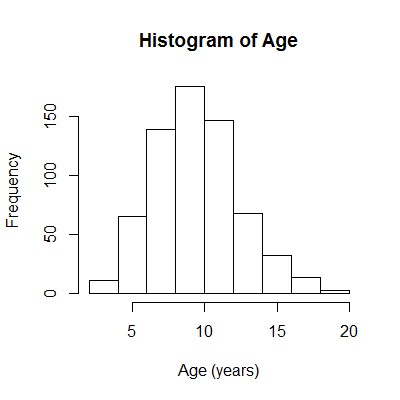
\includegraphics[height=0.6\textheight]{./histogram-age}

\pause
\vspace{-0.45cm} \begin{scriptsize} R code:  \texttt{hist(fev\$age, xlab="Age (years)", ylab="Frequency", main="Histogram of Age")\\} \end{scriptsize}

\end{frame}

% boxplots
\begin{frame}
\frametitle{Univariate Descriptive Statistics: Graphical}

Boxplots are useful for seeing outliers and central location (for a quantitative variable):\vspace{-0.8cm}

\center 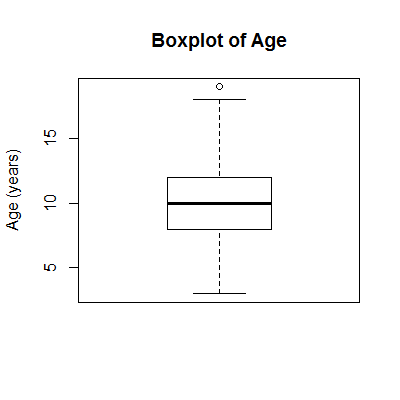
\includegraphics[height=0.7\textheight]{./boxplot-age}

% R code: 
\vspace{-1cm} \begin{scriptsize} \texttt{boxplot(fev\$age, xlab="", ylab="Age (years)", main="Boxplot of Age")} \end{scriptsize}

\end{frame}

% barplots
\begin{frame}
\frametitle{Univariate Descriptive Statistics: Graphical}

Barplots can\footnote[frame]{Sometimes, though, a numerical summary can be more informative: \\ \hfill \texttt{table(fev\$smoke)} = 65 589} be used to summarize categorical variables: \vspace{-0.8cm} % numerical summary = #/prop  in each category (smoke = 65 (9.9%), no smoke = 589 (90.1%))

\center 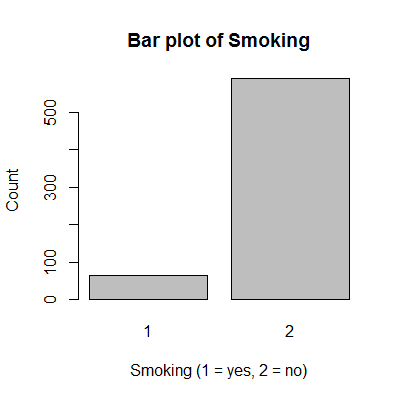
\includegraphics[height=0.6\textheight]{./barplot-smoke}

% R code: 
\vspace{-0.5cm} \begin{scriptsize} \texttt{barplot(table(fev\$smoke), xlab="Smoking (1 = yes, 2 = no)", ylab="Count", main="Bar Plot of Smoking")\\} \end{scriptsize}
\end{frame}

% stratified descriptive statistics
\begin{frame}
\frametitle{Stratified Descriptive Statistics} % useful for categorical vs quantitative comparisons

Sometimes we're interested in the distribution of a variable within certain subgroups, rather than across all the data: \vspace{-0.3cm}
\begin{itemize}
\item e.g., how does the distribution of age differ between smokers and non-smokers in our FEV dataset? % from Monday, how does distribution of FEV differ between teens and pre-teens
\end{itemize}

Stratified descriptive statistics can help us:\vspace{-0.3cm}
\begin{itemize}
\item understand the role of that  stratification variable (e.g., is it a confounder?)
\item begin to demonstrate the association between two variables (one quantitative, one categrical)
\end{itemize}

\begin{footnotesize} \textit{It's often helpful to present stratified descriptive statistics in your ``Table 1" (stratified by outcome or exposure, depending on application). Did the air pollution paper do this?} \end{footnotesize}

% examples in air pollution Table 1
\end{frame}

% stratified histograms
\begin{frame}
\frametitle{Stratified Descriptive Statistics: Graphical}

\vspace{-0.5cm}
\begin{center} 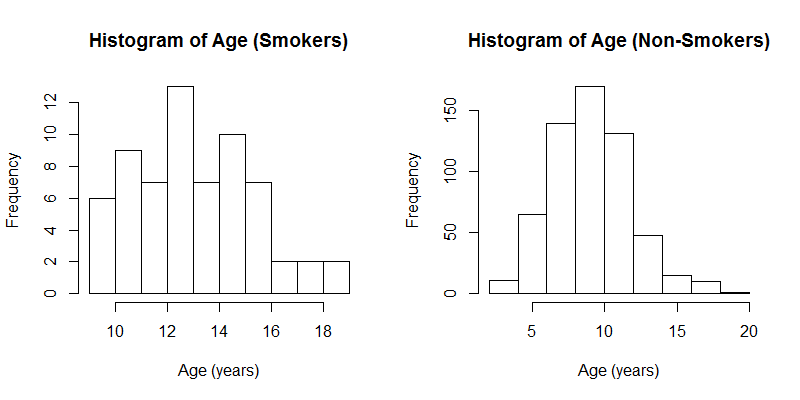
\includegraphics[width=\textwidth]{./histogram-age-stratified} \end{center}

% R code: 
\vspace{-0.75cm} \begin{scriptsize} \texttt{\#plot on left: \\ hist(subset(fev,smoke==1)\$age, xlab="Age (years)", ylab="Frequency", main="Histogram of Age (Smokers)")} \\
\texttt{\#plot on right: \\ hist(subset(fev,smoke==2)\$age, xlab="Age (years)", ylab="Frequency", main="Histogram of Age (Non-Smokers)")\\} \end{scriptsize}
\end{frame}

% stratified boxplots
\begin{frame}
\frametitle{Stratified Descriptive Statistics: Graphical}

You could also use side-by-side boxplots rather than side-by-side histograms (can be easier to compare): 

\vspace{-0.6cm} \center 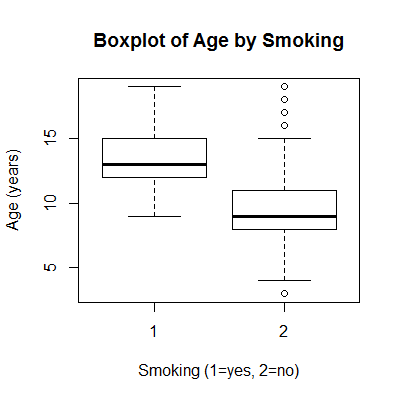
\includegraphics[height=0.6\textheight]{./boxplot-age-stratified}

\vspace{-0.3cm} \begin{scriptsize} \texttt{boxplot(fev\$age $\sim$ fev\$smoke, xlab='Smoking (1=yes, 2=no)', ylab='Age (years)', main = 'Boxplot of Age by Smoking')\\} \end{scriptsize}

\end{frame}

% scatterplot
\begin{frame}
\frametitle{Bivariate Descriptive Statistics}

Scatterplots are a useful tool for summarizing the relationship between two quantitative variables:

\vspace{-0.8cm} \center 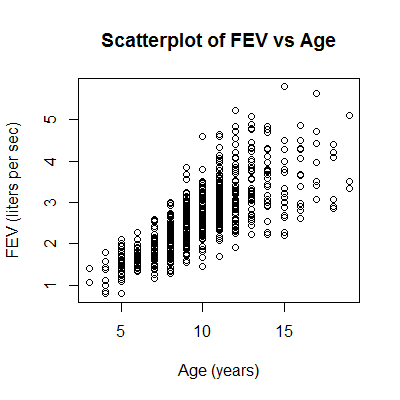
\includegraphics[height=0.65\textheight]{./scatterplot-fev-age}

\vspace{-0.4cm} \begin{scriptsize} \texttt{plot(fev\$fev $\sim$ fev\$age, xlab='Age (years)', ylab='FEV (liters per sec)', main = 'Scatterplot of FEV vs Age')\\} \end{scriptsize}

\end{frame}

% descrip in R
\begin{frame}
\frametitle{Descriptive Statistics in R}

This is just a small taste of the many possibilities when it comes to tools for summarizing data.

We'll spend more time discussing descriptive statistics in Discussion Section next week, including how to generate numerical summaries and graphical summaries like these (or better ones!) in \texttt{R}.

You'll also get practice on your next homework assignment, future assignments, and your data analysis project!

\end{frame}

% descriptive vs inferential stats
\begin{frame}
\frametitle{Descriptive Statistics vs Inferential Statistics}

\color{blue} Descriptive Statistics: \color{black}
\begin{itemize}
\item Goal = \color{blue} describe \color{black} what's happening \color{blue} \textit{in our sample} \color{black}
\end{itemize}

\color{orange} Inferential Statistics: \color{black}
\begin{itemize}
\item Goal = use our data to \color{orange} infer \color{black} something about \color{orange} \textit{our population of interest} \color{black}
\end{itemize}

Often when people talk about ``doing statistics," they're talking about inferential statistics, and this will be the focus of much of our course. \begin{footnotesize} (But, there are many other important components, including study design, translating scientific questions into statistical questions/hypotheses, and descriptive statistics.) \end{footnotesize}

\end{frame}

% intro to statistical inference
\begin{frame}
\frametitle{Statistical Inference}
Why do we do statistics? \vspace{-0.3cm}
\begin{itemize}
\item We can't (usually\footnote[frame]{If we could, then we have no need for inferential statistics!}) measure everyone in our \textbf{population}
	\begin{itemize}
	\item \textit{Example}: all children in the US
	\end{itemize}
\pause
\item Instead, we take a \textbf{sample}
	\begin{itemize}
	\item \textit{Example:} 654 children who came into a particular pediatric clinic for a routine check-up
	\item Note: important to sample well so that the sample truly reflects (is \textit{representative} of) our population of interest
	\end{itemize}
\pause
\item We hope that what we estimate from the sample also applies to the population
	\begin{itemize}
	\item The process of translating from the \textit{sample} to the \textit{population} is \textbf{statistical inference}
	\item What we estimate in the sample = \textbf{estimate} or \textbf{statistic}
	\item Corresponding value in population = \textbf{parameter}
	\end{itemize}
\end{itemize}
\end{frame}

% stat inference: flowchart
\begin{frame}
\frametitle{Statistical Inference: Work Flow} % modify to start with scientific question?

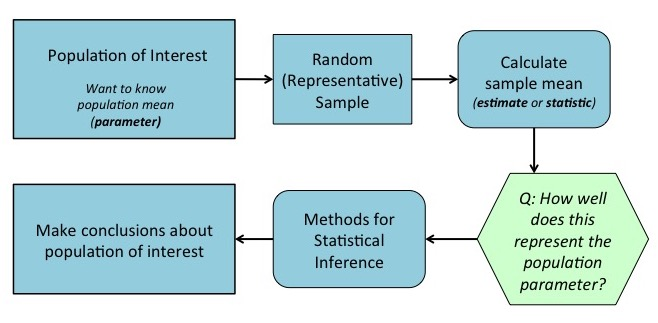
\includegraphics[width=\textwidth]{./inference}

\end{frame}

% stat inference work-flow: FEV example
\begin{frame}
\frametitle{Statistical Inference: FEV Example} % by the end of this class, you should be able to do this!

\begin{itemize}
\item \textbf{Scientific question:} what is the typical FEV for children in the US? \pause
\item \textbf{Statistical question:} what is the average FEV among children in the US? \pause
\item \textbf{Population of interest:} all children in the US \pause
	\begin{itemize}
	\item \textbf{Parameter:} population mean \pause
	\end{itemize}
\item \textbf{Sample:} 654 children who came into a particular pediatric clinic for a routine check-up \pause
	\begin{itemize}
	\item \textbf{Statistic/estimate}: sample mean \pause
	\item[]\begin{footnotesize} \texttt{mean(fev\$fev)} = 2.64 liters per second \end{footnotesize}
	\end{itemize}
\end{itemize}

\vspace{-0.4cm} \textbf{Next step:} use what we see in our sample to draw conclusions about population of interest.\\ \begin{footnotesize}In our sample, the average FEV is 2.64 l/sec. What can we conclude about the population average? Is it \textit{exactly} 2.64 l/sec?\\ \end{footnotesize}

% could have them practice this process with air pollution study? or try it at start of next class? or do it on the HW?
\end{frame}

% precision and inference
\begin{frame}
\frametitle{Precision and Inference}
\begin{itemize}
\item Using descriptive statistics, we can get sample estimates
	\begin{itemize}
	\item e.g., the \textbf{mean} FEV is 2.64 liters per second
	\item e.g., the \textbf{proportion} of kids who smoke is 0.099 (9.9\%)
	\end{itemize}
\pause
\item We want to use these sample estimates to infer something about the population
\pause
\item To assess how well these estimates represent the population of interest, we need to know how \textbf{accurate} and \textbf{precise} they are
	\begin{itemize}
	\item Accuracy: are we estimating the right thing? % on average, will our statitstic be close to the parameter we're trying to estimate? 
	\item Precision: how variable are our estimates? 
	\end{itemize}
\end{itemize}
\vspace{-0.3cm} \textit{Just like we want to describe the center and spread of variables when we summarize our data, we also want to understand the center (accuracy) and spread (precision) of our estimates.}
\end{frame}

% precision and inference
\begin{frame}
\frametitle{Precision and Inference}
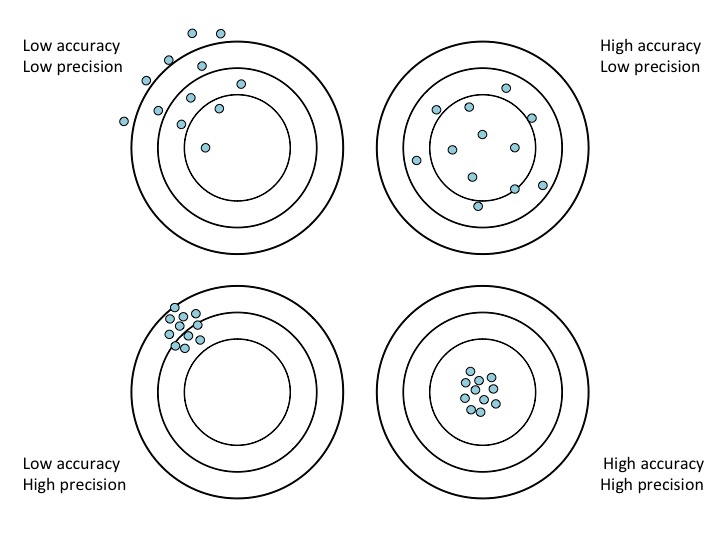
\includegraphics[width=\textwidth]{./accuracy} % start in upper left, describe what each point represents (new estimate from repeated sampling); tie back to this figure when we talk about standard errors and confidence intervals
\end{frame}

% precision and inference
\begin{frame}
\frametitle{Precision and Inference}
How do we know how precise our estimate is?
\begin{itemize}
\item For precision, we need to know how our statistic (estimated from a sample) would vary in repeated samples
\item i.e., if I were to sample from this population another time, how different would the estimate be? And if I sampled from the population a third time, or a fourth time, or...?
\item Our statistics are \textit{random}: the value you get will change depending on which sample you've ended up with
	\begin{itemize}
	\item The \textbf{distribution} of a random quantity describes how that random quantity behaves
	\item The spread of the distribution of our statistic will tell us about the precision of our statistic
	\end{itemize}
\end{itemize}
\end{frame}

% quick detour: probability distributions
\begin{frame}
\frametitle{Probability Distributions}

The \textbf{distribution} of a random quantity tells you what values that quantity can take and how likely it is to take each of those values.

\begin{figure}
\includegraphics[height=0.4\textheight]{./normal-density}
\caption{\color{orange} Area under curve \color{black}= probability that our random quantity takes values between 0.5 and 3}
\end{figure}

\end{frame}

\begin{frame}
\frametitle{Probability Distributions: Normal Distribution}

\begin{center} 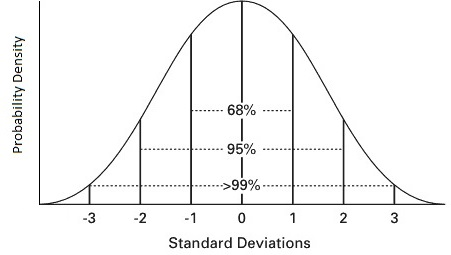
\includegraphics[height=0.4\textheight]{./Normal} \end{center}

\vspace{-0.3cm} \color{blue} Useful property: \color{black} if a random quantity is Normally distributed ($\sim N(\mu,\sigma)$), then 95\% of the time that quantity will take values within two standard deviations ($\sigma$) of its mean ($\mu$)

\begin{footnotesize} (Many of the random quantitites we care about have a Normal distn!)\\ \end{footnotesize}

\end{frame}

% sampling distn = distn of a statistic; center of this distn = accuracy; spread of distn = precision 
\begin{frame}
\frametitle{Precision and Inference: Sampling Distributions}

Recall: \vspace{-0.3cm}
\begin{itemize}
\item We have an estimate, which we've calculated from our sample, and we want to use that estimate to infer something about the general population.
\item To assess how well this estimate represents our population of interest, it's important to know how precise our estimate is. 
\item To figure out the precision of our estimate, it helps to know its distribution.
\end{itemize}

The distribution of an estimate/statistic is called a \textbf{sampling distribution}.

\end{frame}

% sampling distributions: CLT
\begin{frame}
\frametitle{Precision and Inference: Sampling Distributions}

The \textbf{Central Limit Theorem} tells us the sampling distribution of some statistics that we often care about:

\begin{itemize}
\item \textbf{Mean:} For large samples, the sampling distribution of the sample mean is approximately Normal: $\bar{X} \sim N(\mu,\frac{\sigma^2}{n})$
	\begin{itemize}
	\item $\mu =$ population mean
	\item $\sigma =$ population variance
	\item $n =$ sample size
	\end{itemize}
\item \textbf{Proportion:}  For large samples, the sampling distribution of the sample proportion is approximately Normal: $\hat{p} \sim N(p,\frac{p(1-p)}{n})$
	\begin{itemize}
	\item $p =$ population proportion
	\item $n =$ sample size/number of trials
	\end{itemize}
\end{itemize}

\end{frame}

% back to precision: standard error
\begin{frame}
\frametitle{Precision and Inference: Standard Error}

Once we know the sampling distribution of our estimate, it's fairly straightforward to figure out how precise it is.

\color{blue} Example: \color{black} Suppose we have two estimates. The first has sampling distribution $N(2,5)$ and the second has sampling distribution $N(2,1)$. \textit{Which of these estimates is more precise?}

\pause
\begin{footnotesize} (Hint: precision and variance are inversely related) \end{footnotesize}

\pause
We typically describe the precision of an estimate via its \textbf{standard error}. (Standard error = standard deviation of an estimate/statistic.) 

Estimates with \textit{smaller} standard errors are \textit{more precise}! %(so they vary less from sample-to-sample); refer back to bullseye picture
\end{frame}

% sampling distribution of \frac{\bar{X}-\mu}{s}: t
\begin{frame}
\frametitle{Other Sampling Distributions of Interest}

Back to the topic of sampling distributions...

Sometimes we are interested in the statistic $$T = \frac{\bar{X}-\mu}{s},$$ where $s$ is the standard deviation calculated in our sample and $\mu$ is the population mean. 

While the sampling distribution of $\bar{X}$ is Normal, the sampling distribution of $T$ is not. Instead, it follows a $t$-distribution with $n-1$ degrees of freedom, where $n$ is the sample size.

(But, the $t$-distribution is actually very similar to a Normal distribution, especially for large sample sizes...

\end{frame}

% properties of a t-distribution (how it relates to normal, why we care (which stat follows t))
\begin{frame}
\frametitle{Other Sampling Distributions of Interest: $t$}

\center 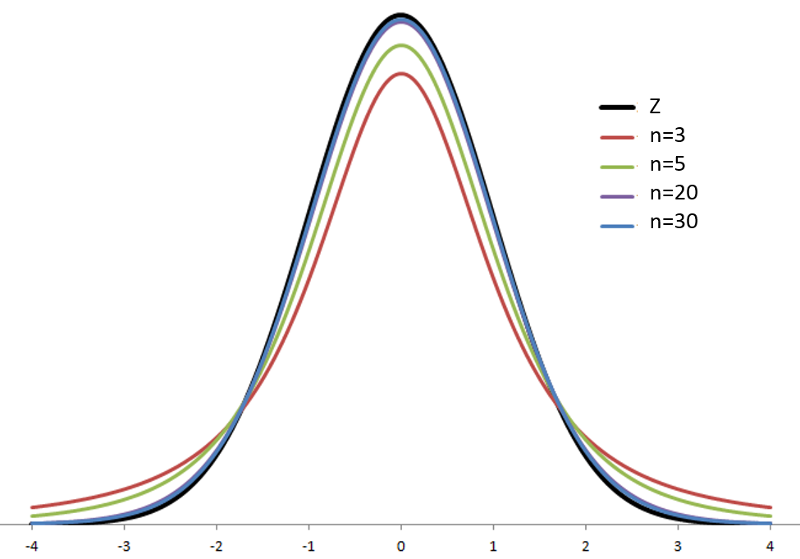
\includegraphics[height=0.8\textheight]{./t-normal}

\end{frame}


% up next: confidence intervals, hypothesis tests
\begin{frame}
\frametitle{What's Next?}

More on statistical inference:
\begin{itemize}
\item Confidence intervals
\item Hypothesis tests
\item Linear regression
\end{itemize}

\end{frame}

% Friday wrap-up
\begin{frame}
\frametitle{``Index Card" \# 2}
On a piece of paper, please write:
\begin{enumerate}
\item Your name
\item Something you learned this week.
\item Something you struggled with this week and/or something you have questions about. 
	\begin{itemize}
	\item[] \begin{footnotesize} (Could be course content, a particular homework problem, course logistics, ..., anything.) \end{footnotesize}
	\end{itemize}
\item Would you find it helpful if we recorded lectures and discussion sections?
\end{enumerate}
Turn in this piece of paper at the end of classs.
\end{frame}


\end{document}
